Il sistema oggetto di studio consiste in un'applicazione distribuita su tre server:
\begin{itemize}
    \item Server A: Gestisce l'autenticazione del cliente, la riserva in magazzino del prodotto, la generazione della ricevuta di acquisto, la pianificazione della spedizione e la finalizzazione dell'acquisto.
    \item Server B: Gestisce la logica di business, ovvero implementa tutte le funzioni di shopping quali la gestione del carrello, la consultazione del catalogo e l'acquisto dei prodotti;
    \item Server P: Gestisce l'elaborazione dei pagamenti.
\end{itemize}

\autoref{fig:abapa} mostra in maggiore dettaglio le mansioni dei servers. Si assume che il server P sia un attore esterno al sistema e dunque sotto una diversa proprietà rispetto ai server A e B. inoltre, Si assumono latenze di rete e think times nulli per studiare le performance del sistema nel contesto di carico più pesante e serrato possibile.

Le richieste elaborate del sistema appartengono a una determinata \textbf{classe}, che ne determina la domanda media di servizio a seconda del server che la deve elaborare. Una stessa richiesta può essere più volte promossa a una classe diversa durante il suo viaggio nel sistema, come illustrato nella \autoref{fig:job_journey_with_classes}.

\begin{figure}
    \centering
    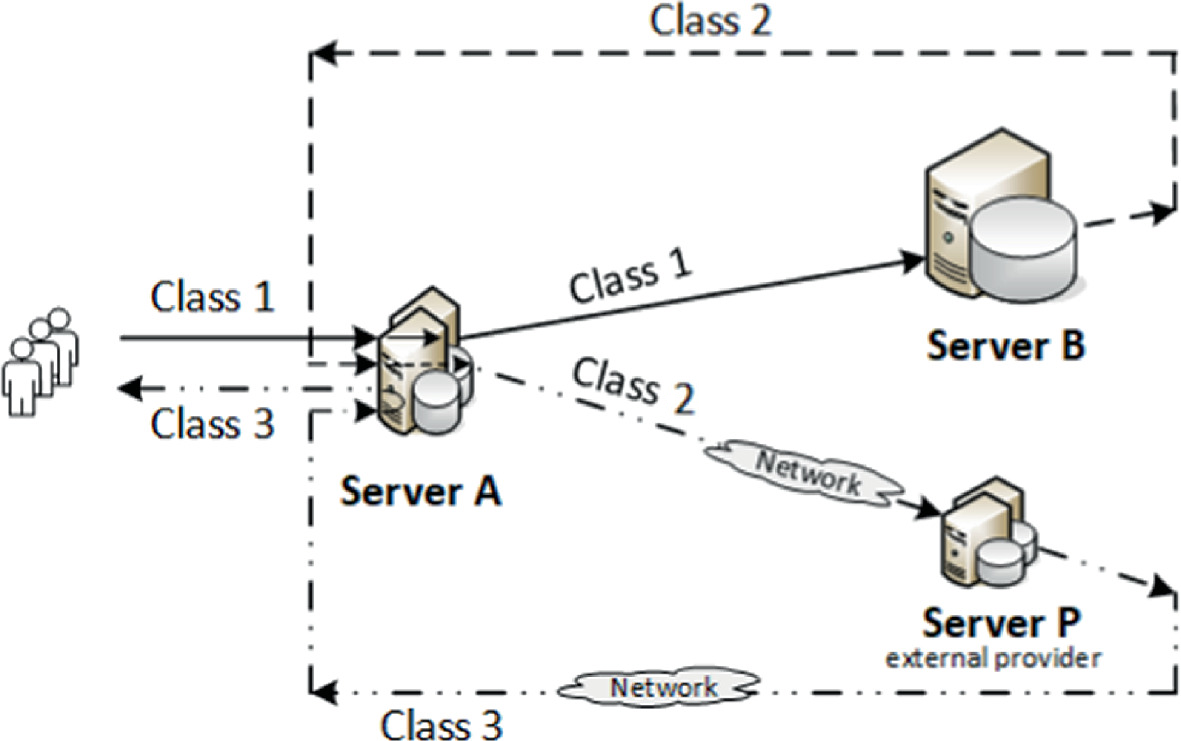
\includegraphics[width=\linewidth]{figs/job_classes.png}
    \caption{Viaggio che le richieste utente intraprendono nel sistema e quali classi vengono loro assegnate \citep{DBLP:books/sp/Serazzi24}}
    \label{fig:job_journey_with_classes}
\end{figure}

\begin{figure}
    \centering
    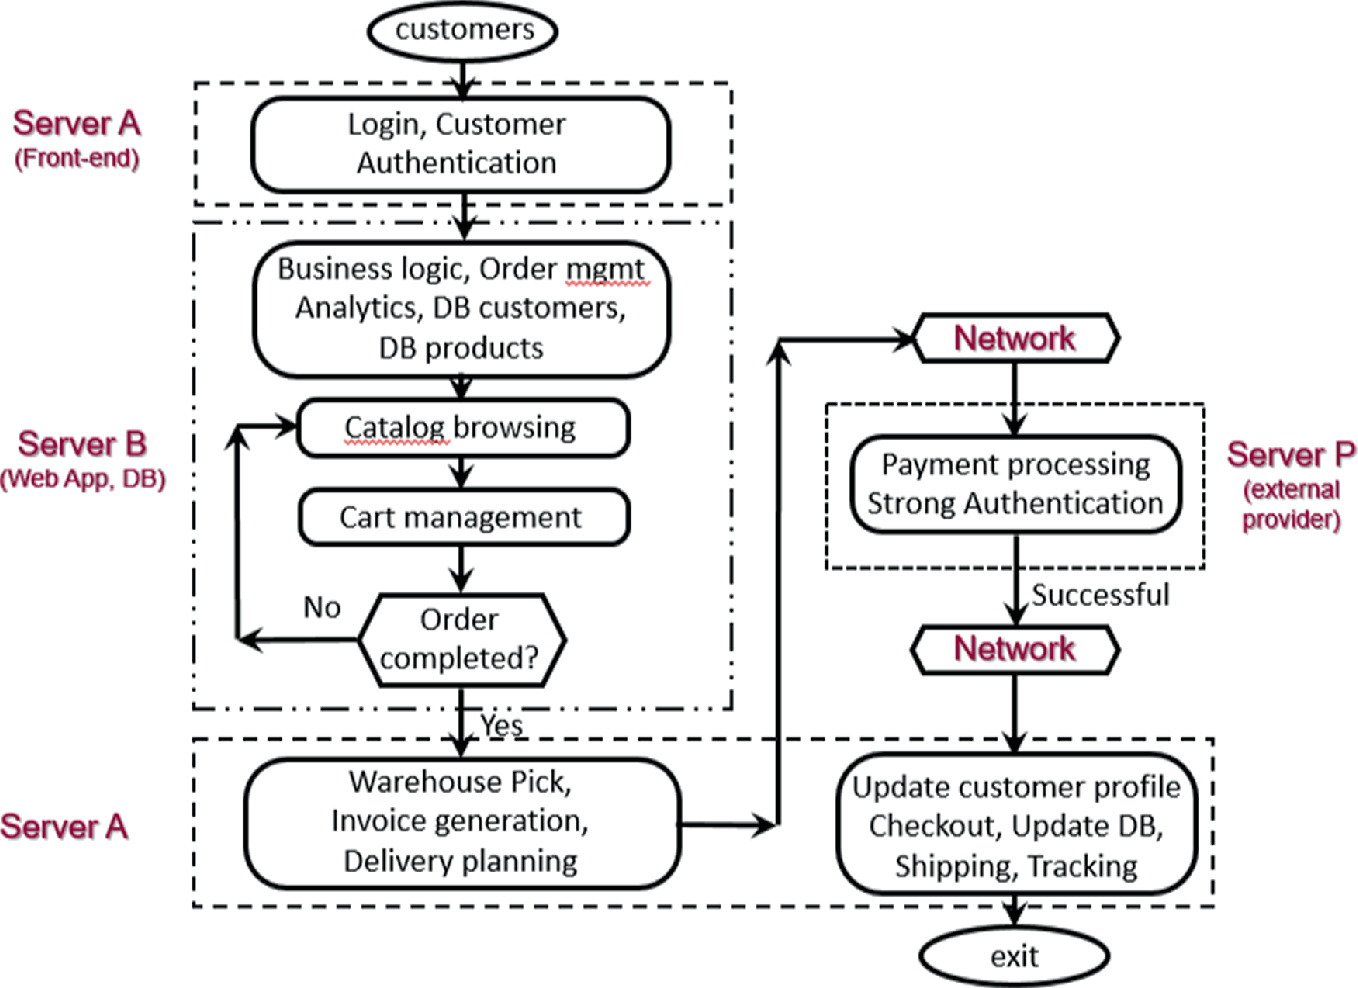
\includegraphics[width=\linewidth]{figs/ABAPA.png}
        \caption{Dettaglio delle mansioni svolte dai server durante le tappe del viaggio di una richiesta all'interno del sistema. \citep{DBLP:books/sp/Serazzi24}}
    \label{fig:abapa}
\end{figure}

